\documentclass[]{article}

\usepackage[utf8]{inputenc}

\usepackage{eurosym}
\usepackage{fullpage}
\usepackage{graphicx}
\graphicspath{{figures/}}
\usepackage[french]{babel}
\usepackage{url}
\usepackage[colorlinks=true, linkcolor=black, urlcolor=blue]{hyperref}
\usepackage{color}
\usepackage[dvipsnames]{xcolor}
\usepackage{titling}
\usepackage{subfig}

\newcommand{\minit}[1]{\noindent{\small\textbf{ \underline{#1}}}\vspace{0.2cm}}
\newcommand{\todo}[1]{\par{\color{red} /---| A faire : #1 |---\textbackslash\\}}
\newcommand{\wordlink}[2]{\hyperref[#1]{#2~\ref{#1}}}

%-- Logos PDG --
\pretitle{
\begin{center}

\begin{figure}[!tbp]
  \centering
  \subfloat{
\includegraphics[width=0.25\textwidth]{UMons_logo.png}}
  \hfill
  \subfloat{
\includegraphics[width=0.25\textwidth]{sciences_logo.png}}\\
\end{figure}
~\newline

}

\posttitle{\end{center}}

\begin{document}

\title{
\vspace{1.6cm}
{\Huge Développement d'un pare-feu domestique}\\
\vspace{0.5cm}
{\Huge Pré-rapport de projet}\\
\vspace{0.2cm}
{\large Activité d' Apprentissage \textsf{S-INFO-037}}\\
}



\author{
\vspace{0.9cm}
\huge{Rémy Decocq}
}

\date{
\vspace{8.5cm}
Année Académique 2018-2019\\
Master en Sciences Informatiques, bloc 1\\
Faculté des Sciences, Université de Mons}

\maketitle          

\thispagestyle{empty}   

\newpage

\tableofcontents
\newpage

\section*{Introduction}
~\\

Depuis maintenant plusieurs années, la connectivité n'a cessé d'évoluer : en se limitant au domaine de l'Internet entre 2000 et 2015, une estimation de l'augmentation du pourcentage de la population mondiale l'utilisant avoisine 40\%  \cite{IWS} \cite{Cable}. Que ce soit dans le cadre d'infrastructures de type "mainframe" ou dans le contexte des ordinateurs personnels, les technologies et équipements relatifs au réseau et aux communications sont devenus indispensables. En conséquence, corrélé au fait de pouvoir de plus en plus s'interconnecter et rejoindre des réseaux de natures variées, le nombre de menaces potentielles pour une machine ainsi connectée augmente grandement. Heureusement, parallèlement à cette évolution, les performances des machines classiques qui en sont équipée ont également suivi une progression en terme de performances. Cela a permis d'en renforcer la sécurité à plusieurs niveaux, et surtout d'intercepter efficacement les menaces étrangères liées à l'utilisation des réseaux. À l'heure actuelle, les OS utilisés classiquement sur des machines desktop fournissent un pare-feu simple (\textit{Windows Defender}, un utilitaire fournit de base dans MAC OS X, \textit{iptables/Netfilter} ou autre pour les distributions Linux). Ce dernier tournant en arrière plan de façon quasi invisible car il demande peu de ressources par rapport à ce qu'une machine actuelle peut offrir.\\

\par En parallèle avec la montée en puissance de ces machines de type desktop, serveurs, etc. s'est développée depuis à peu près les années 2000 la tendance de l'\og Internet des Objets \fg{}, ou encore plus communément abrégé IoT pour \textit{Internet of Things}. Bien qu'assez large, cette dénomination regroupe beaucoup d'objets et de concepts, qu'ils soient virtuels ou non mais possédant un dénominateur commun : la capacité de communiquer en réseau avec d'autres équipements. Cela englobe par exemple la domotique, les outils et capteurs de mesures diverses, les imprimantes et scanneurs en réseau, etc. Tous ces éléments convergeraient idéalement vers une mise en réseau commune, leur permettant de communiquer malgré leur nature hétérogène \cite{Kubler2014}. Cela peut se faire via le réseau Internet, il n'est pas rare d'orienter ces connections vers un cloud permettant de traiter globalement et intelligemment la masse de données qu'il reçoit de ces équipements \cite{Huichen2016}. Or, comme évoqué ci-dessus, plus on s'interconnecte et plus on s'ouvre à des attaquants potentiels, ce qui pose problème si rien n'est mis en place pour s'en protéger.\\

\par Ce travail aura pour objectif premièrement de faire un état de l'art des dispositifs de protection qui sont actuellement déployés dans l'IoT et plus particulièrement dans le cadre domestique. Il s'agit d'un monde beaucoup plus hétérogène et restreint en terme de ressources que celui des ordinateurs qu'on retrouve classiquement dans ce milieu, de fait il n'est pas toujours possible de réutiliser telles quelles toutes les technologies de protection y attenant. De plus, il faut prendre en considération les spécificités d'une habitation : au centre de tous ces équipements communiquant se trouve l'habitant, une personne n'étant pas forcément habilitée à manipuler et contrôler ces nouvelles technologies. Il sera également question d'établir une vision globale des différentes dispositifs de pare-feux existant et sous quelles formes ceux-ci peuvent être implémentés dans les équipements d'une habitation classique. Deuxièmement, il sera question de mettre en pratique ces connaissances pour développer un système en lien avec ces nouvelles mesures de sécurité inhérentes à l'\textit{IoT}. Celui-ci fera intervenir les connaissances acquises au préalables sur les pare-feux.
%http://www.archive.ece.cmu.edu/~ece649/lectures/17_embedded_internet_security.pdf
\newpage
\section{Présentation de l'\textit{Internet des Objets}}\label{IoT}

\subsection{Généralités}

\par L'Internet des objets, qu'on désignera par \textit{IoT} pour le terme plus répandu de \textit{Internet of Things}, est une notion englobant un vaste ensemble de dispositifs. Aucune définition formelle n'est acceptée globalement, mais plusieurs organismes ont tenté d'en établir une ébauche. Par exemple, l'ITU-T (ITU Telecommunication Standardization Sector) Y.2060 le définit comme tel : 
\begin{center}
\textit{“Global  infrastructure  for  the  society,  enabling  advanced  services  by  inter-connecting (physical and virtual) things based on existing and evolving in-teroperable information and communication technologies.”}
\end{center}

\par Derrière cette définition très générale, on peut distinguer plusieurs sous-groupes d'objets connectés distincts, aux applications tant variées que hétérogènes, dans des domaines et secteurs également très différents. C'est ce qui fait la force et en même temps la faiblesse de cet ensemble d'équipements et services qu'on regroupe derrière le terme \textit{IoT} et que des efforts considérables sont déployés pour inter-connecter au maximum. C'est un domaine d'étude intéressant car il représente littéralement ce qu'on pourrait considérer comme le futur de notre environnement technologique. De fait, les équipements que l'ont peut associer à une partie de l'IoT ont déjà fait leur apparition dans notre quotidien : en 2017 on comptait 8,4 milliards de machines en présentant les caractéristiques et les estimations pour l'année 2020 tendent vers 20,4 milliards d'objets connectés d'après la société d'analyse Gartner \cite{Berte2018}.  
\subsection{Caractéristiques des équipements de l'\textit{IoT}}

\subsubsection{Domaines d'application}

Les secteurs dans lesquels l'IoT s'est implanté ces dernières années sont nombreux et très variés : ils s'étendent de l'industrie au domaine des soins de santé en passant par la tendance des \textit{Smart Home}. C'est ce dernier domaine qui est approfondi dans ce travail et qui sera le plus sous-entendu par la suite quand le terme \textit{IoT} est utilisé. La Figure~\ref{domains_IoT} présente une vision d'un schéma global des autres domaines qui gravitent autour du vaste monde de l'IoT.\\


\begin{figure}[!h]
\centering
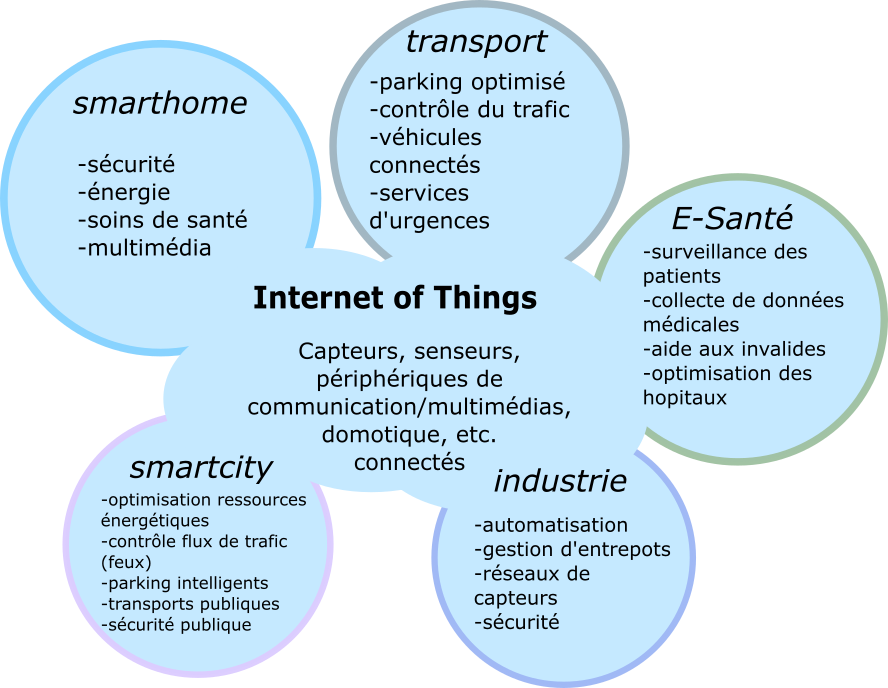
\includegraphics[width=0.6\linewidth]{IoT_domains.png}
\caption{Domaines d'application de l'IoT}
\label{domains_IoT}
\end{figure}

\newpage

\subsubsection{L'environnement \textit{smarthome}}
\par Le terme émergeant \textit{Smart Home/smarthome} est une fois de plus très englobant et général. Il n'en existe pas de définition formelle et communément acceptée. Basman M. Hasan et al. \cite{Basman2016} en présentent plusieurs. Un résultat les unifiant pourrait être
\begin{center}
 \textit{\og Une smarthome est un environnement lié au domicile particulier où plusieurs équipements ou sous-systèmes sont inter-connectés et où les informations qu'ils échangent sont collectées et utilisées afin de surveiller, réguler et automatiser l'écosystème du domicile\fg{}}.\\
\end{center}

\par L'utilisateur en tant que personne physique y vivant est donc au centre de cette architecture, et y siège comme le principal intervenant. Effectivement, l'objectif global du déploiement de tous ces dispositifs est l'amélioration de sa qualité de vie. La notion d'intelligence est intrinsèquement liée avec celle de l'interconnexion de tous ces capteurs et actuateurs déployés dans l'environnement du domicile. Il s'agit d'en récolter et regrouper toutes les données en un point central doté d'une capacité de traitement plus évoluée afin qu'il puisse en tirer une optimisation globale de l'habitation (du système de sécurité, des économies d'énergie, de temps par l'automatisation, etc.).\\

\par Une certaine classification fonctionnelle peut être établie pour distinguer de façon plus concrète les différents équipements qui peuvent intervenir dans l'écosystème d'une smarthome. Elle est schématisée par la Figure~\ref{sm_class}, inspirée de \cite{Basman2016}. Ce qui est désigné par \textit{point d'interconnexion} peut dépendre de l'architecture réelle d'une smarthome \cite{Huichen2016}. Dans la plupart des cas il s'agit d'une machine faisant office de collecteur pour toutes les données transitant dans le domicile et de gateway vers le reste de l'Internet, éventuellement le cloud associé.\\


\begin{figure}[!h]
\centering
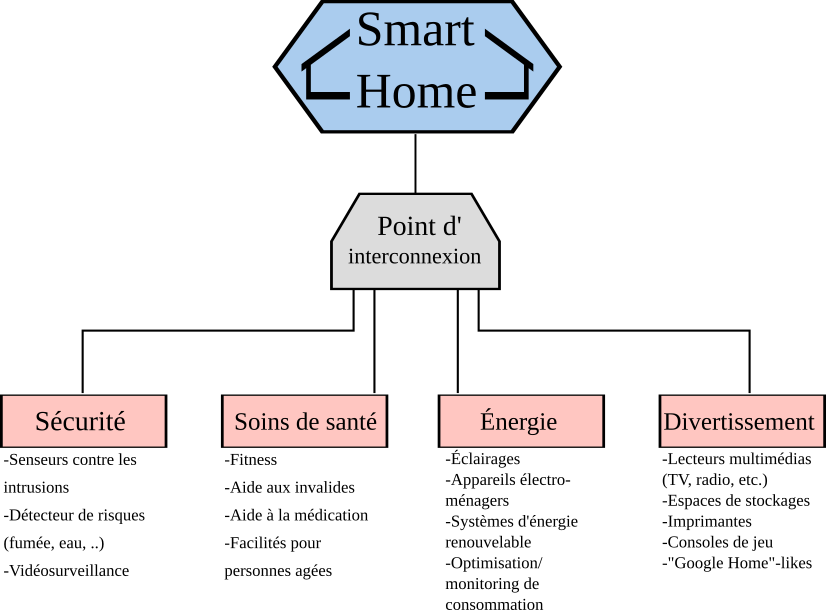
\includegraphics[scale=1.3]{smarthome_class.png}
\caption{Classification fonctionnelle des équipements \textit{IoT} d'une smarthome}
\label{sm_class}
\end{figure}

\newpage

\subsubsection{Exemples d'équipements}

La perception de ce qu'est l'\textit{IoT} par le grand public se résume énormément à l'environnement que constitue la smarthome \cite{Berte2018}. Il s'agit d'une erreur d'incompréhension, on peut tenter de l'expliciter en analysant ce qui compose cette perception. La Figure~\ref{benef_SH} en donne une vision générale (tirée d'un sondage effectué aux États-Unis), qui va être étayée par les exemples concrets d'équipements la suivant.

\begin{figure}[!h]
\centering
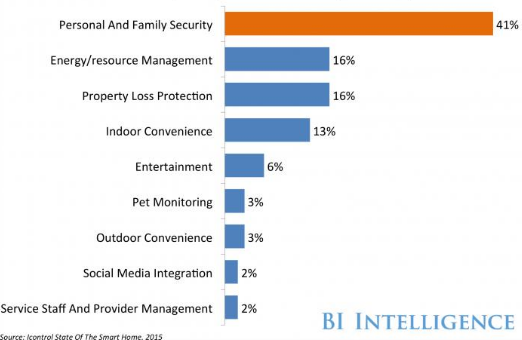
\includegraphics[scale=0.6]{benef_SH.png}
\caption{Top des meilleurs apports des \textit{smarthome} tel que perçu par les Américains}
\label{benef_SH}
\end{figure}

\vspace{0.3cm}
\todo{Remplacer par une section plus pertinente (diff architectures smarthome)}
\minit{Appartenant à la classe sécurité}

\begin{itemize}
\item[$\bullet$] Caméras de vidéosurveillance dites IP
\item[$\bullet$] Systèmes de gestion d'alarme à distance
\item[$\bullet$] Verrous de portes intelligents
\item[$\bullet$] Simulateurs de présence et occupation du domicile
\end{itemize}
\vspace{0.3cm}
\minit{Appartenant à la classe soins de santé}

\begin{itemize}
\item[$\bullet$] Surveillance des patients à leur domicile (contrôle des mesures médicales)
\item[$\bullet$] Accessoires de fitness : montres, balances connectées et autres
\item[$\bullet$] Outils divers d'aide aux personnes invalides (fauteuils, bracelets de secours, ...)
\end{itemize}
\vspace{0.3cm}
\minit{Appartenant à la classe des énergies}

\begin{itemize}
\item[$\bullet$] Luminaires intelligents/automatisés contrôlables à distance
\item[$\bullet$] Frigos, lave-vaisselles, etc. 
\item[$\bullet$] Thermostats connectés, compteurs et senseurs énergétiques
\end{itemize}
\vspace{0.3cm}
\minit{Appartenant à la classe du divertissement \& multimédia}

\begin{itemize}
\item[$\bullet$] Outils de communication : smartphones, babyphones, etc.
\item[$\bullet$] SmartTV, consoles, casques connectés et lecteurs multimédia divers
\item[$\bullet$] Imprimantes et scanneurs en réseau
\item[$\bullet$] Assistants vocaux de maison comme le \textit{google home}
\end{itemize}
\newpage

\subsubsection{Restrictions des équipements}

Malgré le fait que l'ensemble des objets considérés comme appartenant à l'IoT soit très hétérogène, on peut distinguer plusieurs caractéristiques communes à beaucoup d'entre eux. Elles tendent généralement vers ce qui est vu comme une restriction par rapport à un ordinateur type classique (\textit{desktop}). Ces éléments constituent les plus gros freins au développement de la sécurité sur de tels système \cite{Wind2015}. Les conséquences de ces restrictions sont discutées plus en détail dans la \wordlink{prot_IoT}{section} de ce document.\\

\minit{Conçus pour satisfaire une unique fonction}

Le meilleur exemple est celui des capteurs. Un capteur a pour objectif de faire une mesure d'une grandeur physique (température, pression, etc.), d'en tirer une valeur numérique et de faire remonter via son interface avec le réseau cette information vers une unité centrale. Cette dernière accumule ainsi des mesures provenant des nœuds distribués pour y appliquer un traitement, et c'est à ce plus haut niveau que le processus de décision a lieu s'il est nécessaire. Ce genre d'équipement est généralement minimaliste au possible et ne peut donc pas remplir d'autre tâche.\\

\minit{Requièrent une faible consommation énergétique}

Les systèmes embarqués n'ont pas toujours accès à une source illimitée d'énergie, et auront donc une durée de vie limitée à celle de leur batterie. En conséquence, il est souhaitable d'économiser un maximum, ce qui peut se faire en réduisant les temps d'éveil de l'équipement et en optimisant le nombre d'opérations effectuées quand il tourne à plein régime. Dés lors, certains protocoles et algorithmes doivent être adaptés (relatifs aux communications réseaux mais aussi à la sécurité) \cite{Huichen2016}.\\

\minit{Sont contraints en ressources CPU, mémoire et radio}

Ces contraintes sont aussi identiques à celles des systèmes embarqués classiques. En plus de celles-ci, on peut mettre en évidence le fait que les radios (quand il s'agit d'une interface sans fil) sont assez faibles et ne permettent pas des communications à haut débit. En résulte également que des techniques comme le saut de fréquence et les algorithmes de chiffrement de type asymétrique sont plus compliquées à mettre en œuvre \cite{Leloglu2017}.\\


\minit{Sont programmés à un bas niveau d'abstraction}

Étant conçus pour ne remplir que des fonctions spécifiques, certains équipements ne sont pas programmables en utilisant des langages de haut niveau. Par conséquent, ce sont souvent des boîtes noires difficilement manipulables et statiques : les mises à jour et patch de sécurité ne sont pas déployables aisément par les constructeurs \cite{Huichen2016}. Les seules interactions que l'utilisateur lambda peut avoir avec l'équipement sont celles prévues par l'interface de ce dernier s'il y en a une (pour le configurer, consulter son état, etc.).


\newpage

\section{Présentations des pare-feux}

\subsection{Généralités}\label{gen_FW}

Un pare-feu est un dispositif, virtuel ou matériel, qui surveille et contrôle le lien entre un réseau dit de confiance et un réseau extérieur non fiable. Typiquement, ce réseau potentiellement dangereux est Internet et la zone à protéger est le réseau interne d'une entreprise ou d'une habitation. L'existence des pare-feux est une conséquence du besoin d'outils de protection aux bordures de réseaux distincts contrôlés par des entités différentes. D'une part, il faut garantir que des données internes confidentielles restent à l'intérieur du réseau de confiance. D'autre part, il est nécessaire de filtrer les données entrantes et sortantes de ce réseau de sorte qu'aucune menace ne s'y infiltre par des flux, même initiés depuis l'intérieur du réseau de confiance. Ces filtres sont créés et assemblés à partir de \textit{politiques} ou \textit{règles} définies par défaut ou par les personnes compétentes liées à l'entité gérant le réseau.

\subsection{Différentes architectures}

\par Deux classes de pare-feux sont distinguables en fonction de ce qu'ils visent à protéger. La description donnée \hyperref[gen_FW]{en début de section} correspond aux pare-feux au niveau réseau (\textit{network firewalls}), situés en bordure de LANs, WANs et intranets. Ceux-ci, de par leur nature de barrière entre réseaux, peuvent également fournir des services plus évolués : système de NAT, gestion de \textit{zones démilitarisées}, service DHCP, etc. \cite{Shimonski2013} La seconde classe agit au niveau des nœuds du réseau eux-mêmes (\textit{host-based firewalls}), protégeant une machine physique et non pas un réseau entier. Ces pare-feux se présentent donc sous forme de softwares, directement intégrés au niveau du système d'exploitation ou installés à un plus haut niveau.\\

\minit{Les pare-feux niveau réseau}\label{netw_fw}

\par Afin de remplir leur fonction, ces pare-feux sont placés en bordure du réseau à protéger et sont  directement liés aux machines qui font office de \textit{gateway} (routeurs). Tout le trafic passe donc par le pare-feu afin d'être analysé et filtré, ce qui peut représenter beaucoup de données à traiter. Le pare-feu doit offrir une vitesse de traitement proportionnelle aux débits et à la qualité des liens qui le traversent afin de ne pas être un goulot d'étranglement. C'est pourquoi ces pare-feux doivent être très efficaces et sont communément portés (partiellement) au niveau hardware. On parle de \textit{hardware-based firewall appliances}, qui sont des machines physiques dont le seul objectif est de remplir les tâches d'un pare-feu le plus efficacement possible. On y retrouve deux composants : la partie applicative software ou firmware remplissant la fonction de pare-feu, qui repose sur la deuxième partie plus basse constituée de juste ce qu'il faut d'un OS particulier (\textit{jeOS} - \textit{just enough Operating System}). Cet OS est généralement propriétaire, lié au fabriquant du hardware sur lequel les deux parties opèrent et donc optimisé pour garantir les performances requises.\\

\par À plus petite échelle, dans un réseau domestique par exemple, on retrouve également des pare-feux directement implémentés dans le routeur qui fait office de \textit{gateway} pour l'habitation. Ceux-ci sont fatalement moins efficaces et complets que les matériels spécialement dédiés à cette unique fonction.\\

\par À titre indicatif, la Figure~\ref{cisco_FW} donne un exemple d'une \textit{appliance} pare-feu issue de la gamme des Cisco ASA 5500-X (\textit{Adaptive Security Appliance}), la dernière génération que Cisco a introduit sur le marché. Il ne s'agit pas du modèle le plus performant de la gamme en comparant les \href{https://www.cisco.com/c/en/us/products/collateral/security/asa-5500-series-next-generation-firewalls/datasheet-c78-733916.html}{performances et fonctionnalités}, mais convient typiquement bien pour être déployé dans une petite entreprise (son prix avoisine 500\euro). Dans le cas d'une habitation, l'analogue correspondant est dans la majorité des cas le modem distribué par le fournisseur d'accès internet au domicile. La société Proximus fournit par exemple des \textit{b-box}, que leurs clients peuvent configurer par une interface web. Dans ces configurations, il existe bien un onglet intitulé \textit{firewall}, mais celui-ci ne présente que peu d'options de configuration comme le montre la Figure~\ref{proxi_FW}. Dans d'autres onglets, on peut trouver d'autres fonctionnalités qui peuvent y être relatives : restriction d'accès pour certains nœuds en fonction de l'heure (par adresse MAC) et blocage de certains sites par domaine. Cela semble assez faible, les utilisateurs du réseau ont tout intérêt à installer sur leur équipements personnels des \hyperref[host_fw]{pare-feux pour hôtes}.

% https://en.wikipedia.org/wiki/Comparison_of_firewalls
%https://www.cisco.com/c/en/us/products/security/asa-5500-series-next-generation-firewalls/data_sheet_c78-345385.html
\begin{figure}[!ht]
\centering
\begin{minipage}{.4\textwidth}
  \centering
  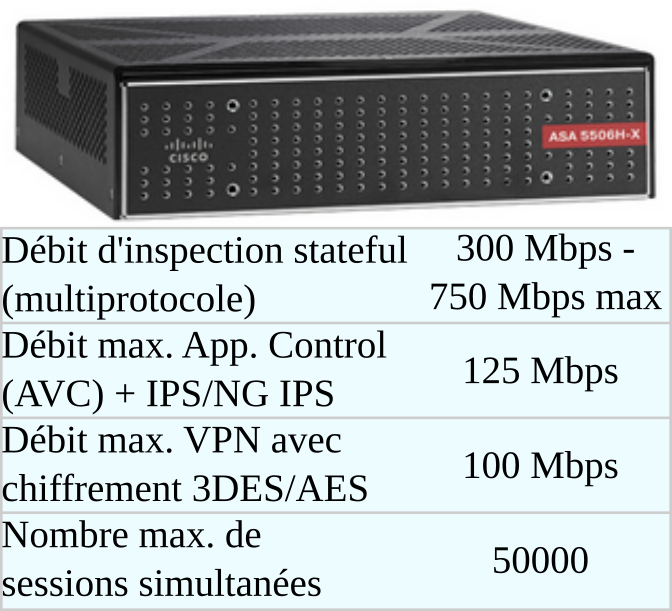
\includegraphics[width=.6\linewidth]{desc_cisco_ASA-5506H-X.png}
  \caption{Cisco ASA 5506H-X}
  \label{cisco_FW}
\end{minipage}%
\begin{minipage}{.6\textwidth}
  \centering
  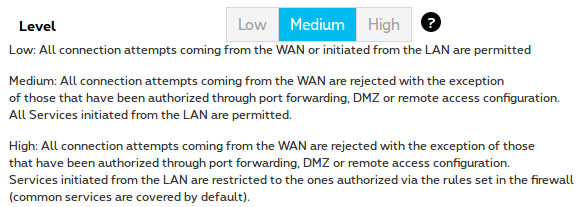
\includegraphics[width=1.0\linewidth]{proximus_FW.png}
  \caption{Options de config. du pare-feu pour une b-box 3V}
  \label{proxi_FW}
\end{minipage}
\end{figure}


\minit{Les pare-feux niveau hôte}\label{host_fw}

\par Du fait que les pare-feux de cette classe sont généralement déployés sur des machines de type desktop, la dénomination \textit{pare-feu personnel} est aussi utilisée. Ces ordinateurs sont généralement munis de tels pare-feux par défaut ou peuvent tout du moins supporter leur installation par l'utilisateur si l'OS utilisé est classique (Windows, MAC OS X, ...). Le pare-feu agit jusqu'au niveau applicatif \cite{Kokko2017} et sous forme d'un \textit{service} ou d'un \textit{daemon} en fonction du système d'exploitation utilisé. Cela permet une proximité étroite avec l'OS et les autres processus. Le pare-feu personnel est donc capable de contrôler le trafic réseau demandé par chaque application et de détecter les menaces engendrées par certains flux. Ces dernières peuvent être entrantes ou sortantes : une machine extérieure qui tente d'établir une connexion suspecte ou un exécutable sur la machine à protéger qui initie un trafic avec une cible blacklistée, par exemple.\\

%https://www.itprotoday.com/security/personal-firewalls
%https://en.wikipedia.org/wiki/Personal_firewall

\par Les principales fonctionnalités d'un pare-feu personnel devraient être au minimum les suivantes \cite{Shimonski2013}
\vspace{0.1cm}
\begin{itemize}
\item[$\bullet$] Bloquer les attaques et comportements dangereux du réseau extérieur : scanning des ports ouverts, attaques par fragmentation, \textit{IP Spoofing}, etc.   
\vspace{0.2cm}
\item[$\bullet$] Stopper les menaces venant de l'intérieur : un exécutable comme un \textit{malware} ou un \textit{spyware} qui tente d'établir une connexion vers l'extérieur doit être bloqué et mis en quarantaine
\vspace{0.2cm}
\item[$\bullet$] Présenter de l'automatisation car d'une part car un utilisateur non-expérimenté pour sa configuration doit quand même rester protégé et d'autre part il doit pouvoir se mettre à jour automatiquement
\vspace{0.2cm}
\item[$\bullet$] Agir au niveau applicatif : un malware pourrait utiliser le port web 80 pour se répandre par exemple, pour détecter cela il faut analyser les payload des paquets et disposer d'une base de données à jour pour y déceler des patterns malicieux
\vspace{0.2cm}
\item[$\bullet$] Alerter l'utilisateur quand un événement survient, et le logger avec suffisamment d'informations pour qu'il puisse prendre une décision adaptée
\vspace{0.2cm}
\item[$\bullet$] Éviter les \textit{faux-positifs} (bloquer du trafic légitime)
\end{itemize}
\vspace{0.5cm}
\par Que ce soit en entreprise ou dans une habitation, il est donc probable que l'on retrouve des pare-feux appartenant à ces deux classes distinctes là où ils sont efficaces (voir  \wordlink{netw_IDS}{Figure}). Il ne s'agit que d'échelles différentes, qui impliquent également des intervenants différents. En entreprise, l'administrateur sécurité/réseau configure du matériel spécifique afin de sécuriser les frontières de son réseau tout en préservant ses performances. Il est aussi possible qu'il installe dans les machines internes de son réseau des pare-feux assez puissants pour empêcher les propagations des attaques déclenchées. Dans le domicile, l'habitant est sommairement protégé par le routeur fournit par son FAI qui inclut un pare-feu réseau par défaut. S'il est un minimum expérimenté, il sera à même d'installer et configurer des pare-feux personnels sur chacun de ses équipements connectés.   


\begin{figure}[!h]
\centering
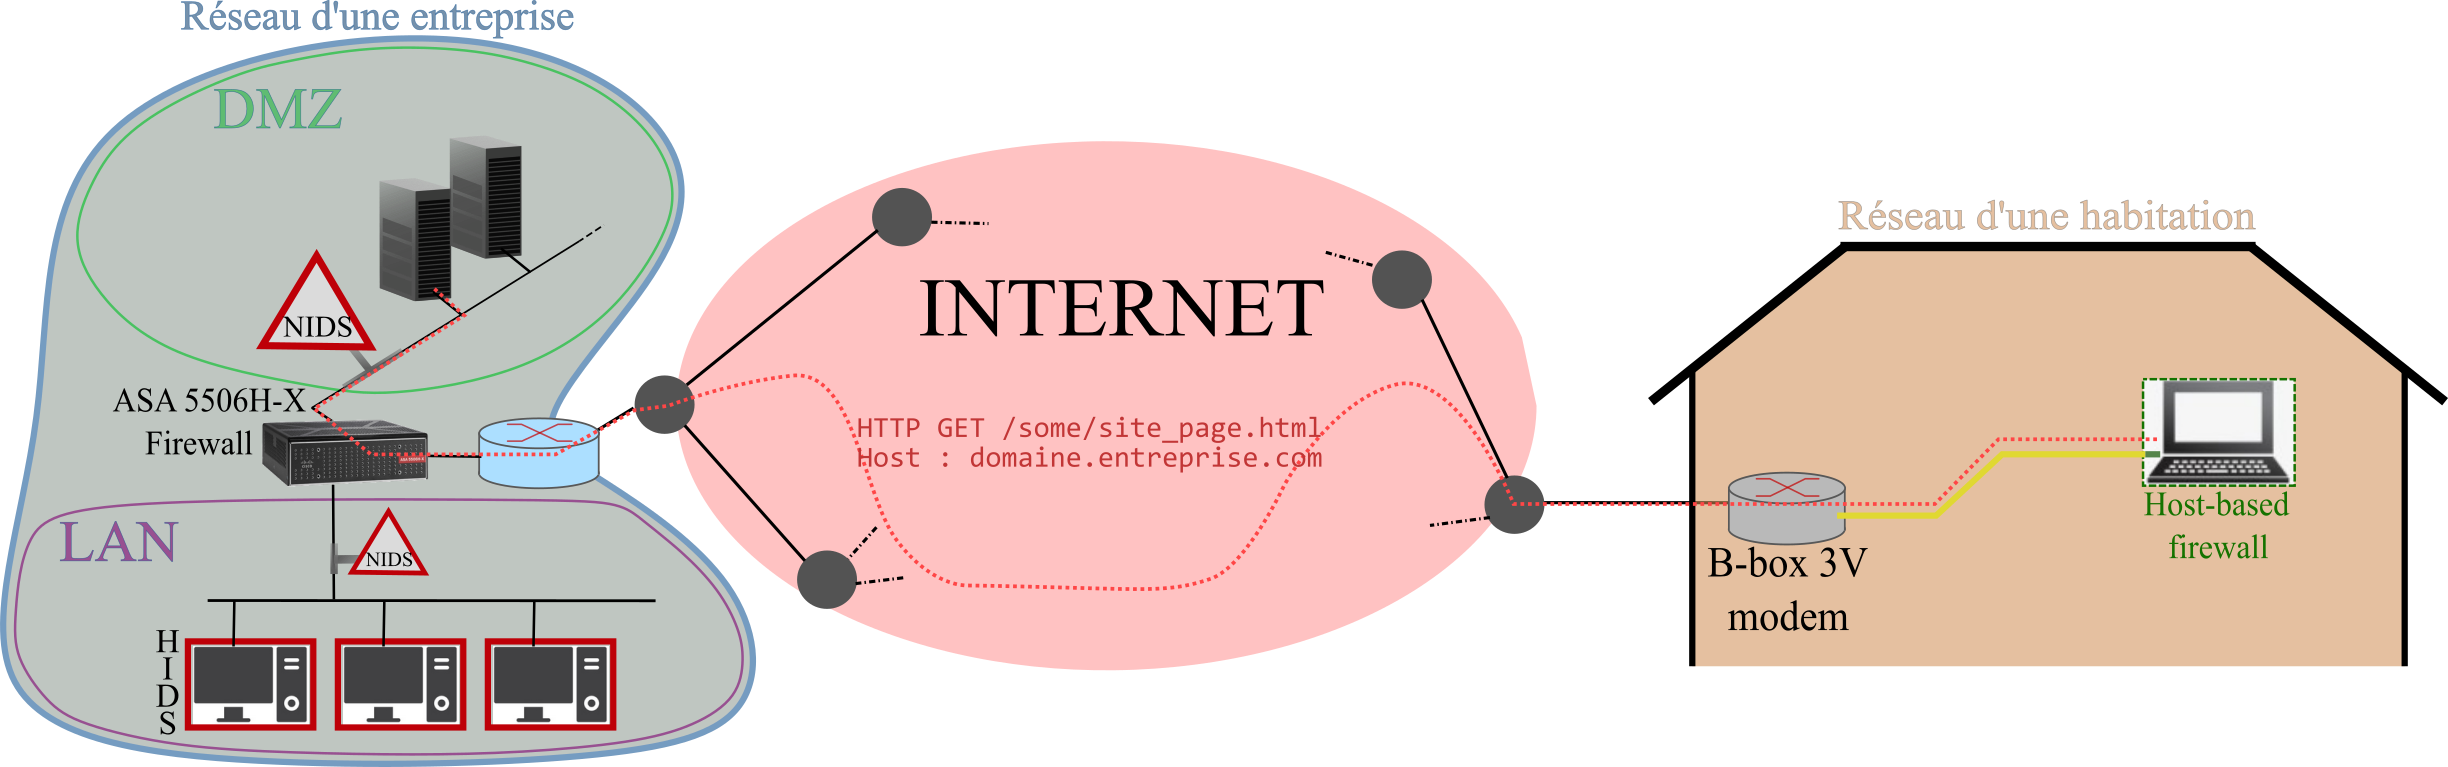
\includegraphics[scale=1.65]{netw_IDS.png}
\caption{Schéma récapitulatif des places des différents dispositifs de protection dans un réseau}
\label{netw_IDS}
\end{figure}

\subsection{Types de pare-feu}

\subsubsection{Pare-feu de filtrage (sans état)}

Aussi désigné dans la littérature par le terme \textit{stateless}. Il s'agit des pare-feux les plus rudimentaires dont le premier prototype remonte à celui élaboré par Jeffery Mogul en 1989 \cite{Shieha2014}. Généralement, ces pare-feux sont rapides mais peu efficaces car facilement dupés. Un pare-feu de ce type inspecte chaque paquet individuellement et détermine s'il peut passer sur base d'un certain ensemble de règles écrites que ses headers matchent ou non. Il s'agit des headers TCP/IP (également UDP), des options y attenant et de l'interface d'entrée principalement. Plus en détail : les adresses IP source et destination, les ports source et destination au minimum seront soumis aux filtres du pare-feu. Il y a plusieurs problèmes avec cette approche :
\vspace{0.2cm}
\begin{itemize}
\item[$\bullet$] Il n'y a aucune vérification au dessus de la couche transport : la partie applicative peut contenir n'importe quoi
\vspace{0.2cm}
\item[$\bullet$] Le pare-feu n'est pas dynamique : il n'apprend rien du trafic qu'il laisse passer. Aucun état n'est retenu, alors que TCP est un protocole lié à une machine à état dont il pourrait être possible de garder une trace
\vspace{0.2cm}
\item[$\bullet$] Les règles sont très redondantes à écrire pour être efficace, très peu modulables et facilement sujettes aux erreurs et oublis
\end{itemize}
\vspace{0.25cm}

Les paquets ICMP peuvent également faire l'objet d'un filtrage du même acabit \cite{Shimonski2013}.
Ce type de pare-feu tombe en désuétude car ils sont trop simples à duper par des attaquants.  

\subsubsection{Pare-feu à état}

Le but de ce type de pare-feu dit \textit{stateful} est d'améliorer les techniques de filtrage sans état en maintenant de l'information sur les flux passant au travers, principalement TCP. Effectivement, au contraire d'UDP, TCP est un protocole qui garde un état qui se traduit dans certains champs de ses headers. Dès lors, le pare-feu peut accéder à cette information, l'analyser et l'utiliser pour en déduire dans quel état est actuellement la connexion entre les deux processus communiquant sur les deux hôtes impliqués. Cela peut se traduire par l'inspection des flags (SYN, FIN, ...), des numéros de séquences et acquittements qui permettent au pare-feu de contrôler en conséquence le contenu d'une table interne des connexions.\\ 

\par L'établissement d'une connexion se fait comme suit : lors de la réception du premier paquet TCP par le pare-feu, celui-ci va le soumettre à ses règles de filtrage définies comme dans un pare-feu sans état. Si le paquet est valide, il est retransmis pour poursuivre librement sa route et une entrée est ajoutée dans la table interne du pare-feu. Celle-ci va changer d'état à chaque paquet de la communication reçu, jusqu'à arriver dans un état \textit{established} correspondant à la fin du 3-way handshake TCP. Tous les paquets suivants pourront alors être traités rapidement en faisant matcher les headers à ceux de l'entrée en état \textit{estbalished} dans la table (qui sont donc théoriquement également légitimes). Cette façon de procéder est plus efficace que de soumettre chaque paquet individuellement aux règles de filtrage qui peuvent être complexes et demander beaucoup de travail et donc gourmandes en temps.\\

\par Dans le cas d'une communication utilisant UDP, le contrôle possible est moins fin car il ne s'agit pas d'un protocole à état et les échanges ne sont pas bidirectionnels. Dans ce cas, lorsque le premier paquet d'une transmission arrive en entrée du pare-feu, il est soumis aux règles de filtrage. S'il est considéré comme correct, le pare-feu ajoute une entrée dans sa table pour les couples d'adresses et ports et considérera les suivants comme légitimes. Cette entrée expirera après un temps donné sans autre nouveau paquet la matchant. 



\subsubsection{Pare-feu applicatif}\label{appfw}

\par Ce type de pare-feu peut être considéré comme une extension complète aux simples pare-feux à états dans le but d'en améliorer la fiabilité. Là où ces derniers sont capables de déterminer quels protocoles sont utilisés et autorisés sur chaque port, les filtres ajoutés au niveau applicatif peuvent en plus déduire à quelles fins sont utilisés ces protocoles (l'inspection va jusqu'à la couche 7 du modèle OSI). Il s'agit cependant de plus que de simples filtres, c'est une technologie à part entière qui est utilisée : l'inspection profonde des paquets ou \textit{deep packet inspection} (DPI). Les pare-feux utilisant la DPI mêlent les fonctionnalités d'un pare-feu à état avec les systèmes de détection et prévention d'intrusions (sous-sections~\ref{IDS} et \ref{IPS}). La décision de bloquer ou de laisser passer le paquet tient compte de ce qu'il contient réellement au niveau données et de l'interprétation qui en est faite pour déterminer s'il représente un danger.\\

\phantomsection
\label{waf}
\par Par exemple, les \textit{Web Application Firewalls} (WAF) sont une sous-catégorie des pare-feux applicatifs qui opèrent un filtrage sur le trafic HTTP. Ils peuvent donc filtrer le trafic sur base de certaines règles d'accessibilités fixées en bloquant des requêtes aux URL douteuses ou considérées comme non éthiques vis-à-vis de l'organisme maintenant le réseau par lequel elles transitent. Outre cela, les WAFs permettent également de se protéger contre les attaques dites de type \textit{parameter tampering} (injection SQL, cross-site scripting, etc.) \cite{Palka2011}, ainsi que d'inclure des filtres anti-spam pour les courriels \cite{wikifwFR}.\\

\par Plus généralement, les pare-feux applicatifs permettent de se protéger des virus, vers et tentatives d'\textit{exploits} de faiblesses connues des systèmes à protéger \cite{wikiappfw} \cite{Palka2011}. Un autre avantage d'analyser jusqu'à la couche 7 grâce à la DPI est que certains protocoles (FTP par exemple) utilisent la couche applicative pour transmettre des informations relatives aux couches plus basses (adresses IPs, ports, etc.) et qui seront impliquées dans des communications passant par le dispositif pare-feu \cite{wikifwFR}. Comme illustré par l'exemple des WAFs, le principal défaut inhérent à leur nature réside dans le fait que pour chaque type de trafic applicatif que l'on souhaite contrôler, un travail spécifique doit être opéré (établir des règles dédiées par exemple) \cite{wikifw}. 

\subsubsection{Pare-feu applicatif proxy}

Ces pare-feux mêlent l'inspection au niveau applicatif et le rôle de proxy pour les flux qui sont destinés à le traverser originellement. Ainsi, il devient réellement un intermédiaire entre les deux partis communiquant, interceptant les paquets pour les analyser puis les retransmettant vers le destinataire comme s'il en était la source \cite{Shimonski2013}. Avant cette retransmission, le paquet peut être inspecté du point de vue de toutes ses couches et déterminé comme étant dangereux en fonction des opérations de filtrages effectuées dans le proxy. Un contrôle très fin peut donc être opéré. Cela garantit un niveau de sécurité plus haut que les pare-feux de filtrage pur qui traitent les paquets à la volée \cite{frameIP}.\\

\par Cette approche possède cependant trois gros désavantages : 
\begin{itemize}
\vspace{0.2cm}
\item[$\bullet$] Clairement, l'impact sur les performances du réseau n'est pas insignifiant (surtout si le pare-feu n'est basé que sur du software pur et pas sur une machine adaptée)
\vspace{0.2cm}
\item[$\bullet$] À chaque nouveau protocole applicatif que l'on souhaite pouvoir filtrer de la sorte, un nouveau dispositif proxy correspondant doit être pensé et développé pour en inspecter le trafic
\vspace{0.2cm}
\item[$\bullet$] Si un proxy présente une faille de sécurité, un assaillant peut l'utiliser comme un vecteur d'attaque et prendre le contrôle du système sur lequel il tourne. S'il parvient alors à désactiver les services relatifs au pare-feu, la voie vers ce qu'on souhaitait protéger se retrouve toute ouverte
\end{itemize}


\subsubsection{Pare-feu identifiant}\label{idfw}

Pour ce type de dispositif, on veut pouvoir définir des règles de filtrage en fonction de l'utilisateur ou le groupe qui se cache derrière un paquet ou un flux. Plusieurs schémas d'association existent, définissant ce à quoi la notion d'un utilisateur correspond. Par exemple certains de ces pare-feux comme \href{http://www.openbsd.org/faq/pf/authpf.html}{authpf} sous OpenBSD, qui étant placés sur un gateway, exigent qu'avant d'autoriser un flux, l'utilisateur d'un hôte communiquant doit établir une connexion SSH avec ce dernier. Un autre type d'association possible peut se faire par adresse MAC.\\

\par Les pare-feux destinés aux entreprises développés par Cisco (ASA) \cite{cisco2018} et Palo Alto Networks \cite{Kokko2017} utilisent des gestionnaires d'annuaires d'utilisateurs basés sur les services \href{https://fr.wikipedia.org/wiki/Active_Directory}{Windows Active Directory}. Dans ces base de données utilisateurs, on retrouve les différentes adresses IP associées à un utilisateur particulier ainsi que les groupes qu'ils composent. Les interactions avec le pare-feu sont transparentes à ce niveau, en effet ce dernier travaille avec les objets \og utilisateurs \fg et non plus directement les IPs (bien que cela reste possible). Procéder de cette façon apporte plusieurs avantages \cite{cisco2018}:
\vspace{0.2cm}
\begin{itemize}
\item[$\bullet$] Cela simplifie la création et la gestion des politiques de sécurité du pare-feu
\vspace{0.2cm}
\item[$\bullet$] Offre la possibilité d'identifier facilement les utilisateurs utilisant le réseau
\vspace{0.2cm}
\item[$\bullet$] Simplifier la surveillance des activités des utilisateurs du réseau et identifier la source de menaces
\end{itemize} 


%https://www.frameip.com/firewall/
\subsection{Systèmes de détection d'intrusion (\textit{IDS})}\label{IDS}
%https://www.ibm.com/developerworks/library/se-intrusion/index.html
%https://www.comparitech.com/net-admin/network-intrusion-detection-tools/
Ce type de système, abrégé par IDS pour \textit{intrusion detection system}, est analogue à un ce qu'est un système d'alarme intérieur dans l'environnement d'une habitation : quand les dispositifs de protection mis en place à l'entrée sont contournés (une présence non permise est détectée à l'intérieur), l'alarme est lancée et des actions sont éventuellement prises en conséquence. Les IDSs sont donc des sentinelles qui surveillent le réseau interne, logiquement placées après le pare-feu dans le sens entrant. Ces systèmes se présentent sous la forme d'outils spécialisés dans l’interprétation des logs des routeurs, pare-feux, serveurs et autres agents du réseau interne. Les IDSs sont épaulés par une base de données des signatures d'attaques déjà connues et y comparent le contenu des logs afin de trouver des \textit{patterns} qui matchent. Dans une telle situation, plusieurs actions allant de simplement alerter l'administrateur réseau à couper les accès réseaux des machines peuvent être déclenchées, en fonction du degré de certitude (match fort entre les patterns) et de la menace.\\

\par Tout comme les pare-feux, les IDSs peuvent être des ressources software ou reposer sur du hardware spécifique. Dans le cas ou il s'agit de software, ils sont établis sur la même machine que le pare-feu, les proxys ou autres dispositifs de bordure de réseau. S'ils se présentent sous forme d'équipements hardwares spécifiques, ils sont installés de sortes à contrôler et surveiller de près un de ces dispositifs sensibles. Le trafic tant entrant que sortant peut être analysé par les IDSs, car les attaques peuvent autant venir de l'extérieur que se déployer depuis l'intérieur.\\

\par L'analyse des événements repose communément sur deux techniques. La première, la détection par signature (\textit{signature detection}), utilise une base de données de signatures d'attaques déjà connues et se base sur le trafic et les patterns observés pour établir un match avec ces signatures. La seconde approche est celle de la détection d'anomalies (\textit{anomaly detection}). Il est question d'utiliser des heuristiques afin de distinguer les situations et comportements anormaux, sur base de profils types construits par analyses statistiques, agencements de règles ou réseaux neuronaux. Outre la technique utilisée, trois catégories d'IDSs existent en fonction de leur place dans l'architecture réseau (leur mode de fonctionnement diffère en conséquence) :
\vspace{0.3cm}
\begin{itemize}
\item[$\bullet$] Surveillance du réseau (\textit{NIDS}:\textit{ Network-based IDS})
\item[$\bullet$] Surveillance des systèmes du réseau (\textit{HIDS}:\textit{ Host-based IDS}) 
\item[$\bullet$] Surveillance distribuée du réseau (\textit{NIDS}:\textit{ Distribued IDS}) 
\end{itemize} 
~\\
\minit{Les NIDSs}

\par Ces dispositifs surveillent le réseau ou un segment de ce réseau, sous forme d'un équipement intermédiaire de capture (ses interfaces sont en mode écoute pour l'entièreté du trafic transitant par le segment). Il est important d'avoir plusieurs unités de surveillance distinctes dans le cas où le réseau est scindé en plusieurs modules/zones. Par exemple, un serveur web d'une entreprise pourrait être infecté et servir de plateforme de lancement d'une attaque depuis le réseau interne, vers un autre module contenant des serveurs internes.\\

\par Deux manières de procéder à l'analyse sont possibles : soit en mode \textit{in-line} soit en \textit{off-line}. Le cas de la capture du trafic par interface décrit ci-dessus correspond au mode in-line. Le trafic est analysé en temps réel, ce qui permet une plus grande réactivité mais peut constituer un goulot d'étranglement si le processus de décision est coûteux. Le mode off-line est donc plus avantageux à ce niveau, puisque le processus d'analyse et décision est opéré sur des données stockées et non pas à traiter à la volée. Une inspection plus fine est alors envisageable, cependant le principal défaut de ce mode de fonctionnement reste le manque de réactivité à une attaque.

~\\
\minit{Les HIDSs}

\par Les IDSs orientés systèmes sont élaborés dans le but de protéger uniquement l'hôte sur lequel ils sont déployés. Ils ciblent également de façon précise le trafic qu'ils doivent surveiller en fonction de la nature du système. Par exemple, si l'hôte ne maintient aucun service DNS, il est inutile d'analyser des requêtes DNS qui lui parviendraient pour y déceler un menace exploitant une faille connue dans le protocole DNS. Puisque les HIDSs vont s'exécuter sous forme d'un processus (\textit{daemon}) sur la machine hôte qui elle-même fonctionne sous un OS classique, un lien doit être établi entre les deux pour que l'HIDS puisse surveiller le système et les interfaces réseaux. Certains vont même jusqu'à rechercher les intrusions dans le noyau de l'OS.\\

\par D'une part, un HIDS peut surveiller le comportement du système  dynamiquement en récupérant des informations que ce dernier met à sa disposition à la manière d'un antivirus. Différents indicateurs sont à interpréter :
\vspace{0.2cm}
\begin{itemize}
\item[$\bullet$] Activité de la machine même : processus qui y vivent, ressources qu'ils consomment (CPU, RAM, réseau etc.), modification dans les comptes utilisateurs
\vspace{0.2cm}
\item[$\bullet$] Activité des utilisateurs : commandes entrées, programmes lancés, tentatives d'accès à des ressources non autorisées, passage au compte administrateur
\vspace{0.2cm}
\item[$\bullet$] Patterns d'exécution ou de procédure de déploiement des vers, virus, chevaux de Troie (shell ouvert simultanément à l'ouverture d'un fichier, accès anormaux aux interfaces réseau, ...)
\end{itemize}
\vspace{0.4cm}
\par D'autre part, certaines sections plus critiques du système peuvent être intéressantes à analyser finement, car c'est généralement là qu'un attaquant voulant prendre le contrôle de la machine va laisser des traces en y installant ses outils softwares. Un HIDS voulant s'assurer que des sections critiques (système de fichiers, registres, ...) ne sont pas infectées va maintenir une base de données de leur évolution dans le temps, sous forme d'attributs et sommes de contrôles (\textit{checksums}). Ces dernières permettent d'assurer l'intégrité des ressources concernées en en comparant les valeurs régulièrement dans le temps, et notifiant les différences observées.

~\\
\minit{Les DIDSs}
%https://www.symantec.com/connect/articles/introduction-distributed-intrusion-detection-systems
\par Les DIDSs se présentent sous la forme d'une architecture distribuée d'IDSs (surveillant des segments de réseaux et/ou hôtes), et d'une unité centrale de management qui récolte toutes les informations de ces dispositifs déployés. Ainsi, la machine centrale peut maintenir une vaste base de données centralisée, représentant l'état global du réseau à protéger. Cette approche présente plusieurs 
avantages :
\vspace{0.2cm}
\begin{itemize}
\item[$\bullet$] moins de faux positifs car plus de données pour justifier une prise de décision (agrégation des événements et attaques)
\vspace{0.2cm}
\item[$\bullet$] mises à jour et distribution de la base de données des signatures aisées
\vspace{0.2cm}
\item[$\bullet$] centralisation des alertes/logs, contrôle global avec une vue d'ensemble
\vspace{0.2cm}
\item[$\bullet$] réponses aux événements plus efficaces, IDSs plus simples à administrer en conséquence (ajout de nouvelles règles suite à des brèches découvertes, blacklisting d'IPs, etc.)
\end{itemize}
\vspace{0.4cm}

\par Afin de transmettre les alertes générées jusqu'à l'unité centrale efficacement, les différents nœuds IDSs du réseau devraient communiquer de façon homogène. À cette fin, un standard a été écrit sous le nom de format IDMEF (\textit{Intrusion Detection Message Exchange Format}, RFC 4765). Ce langage d'alertes est lisible par l'humain, utilisant le format XML. Utilisé par tous les nœuds qui effectuent la tâche de détection d'intrusion (quelque soit le type et l'implémentation), l'unité centrale qui récolte toutes les alertes peut utiliser un outil de pilotage de la sécurité du réseau global comme \href{https://fr.wikipedia.org/wiki/Prelude_SIEM}{Prelude}. Cet outil normalise, trie, agrège, corrèle et en tire les conclusions sur des décisions à prendre pour protéger le réseau, tout en fournissant une interface (et des logs) via laquelle l'administrateur peut surveiller ce qui se passe globalement.

\subsection{Systèmes de prévention d'intrusion (\textit{IPS})}\label{IPS}
%https://fr.wikipedia.org/wiki/Syst%C3%A8mes_de_d%C3%A9tection_et_de_pr%C3%A9vention_d%27intrusions_dans_les_syst%C3%A8mes_distribu%C3%A9s
\par Dans la section précédente, il était question de détection des attaques et pour certaines d'entre elles des actions à effectuer en contre-mesure pour bloquer la menace. Cela relève du domaine d'application des systèmes de prévention d'intrusion, aussi abrégé IPS pour \textit{intrusion prevention systems}. Tout comme pour les IDSs, deux types d'IPS peuvent être distingués en fonction de leur place dans l'architecture réseau : les \textit{host-based IPS} agissent au niveau local pour un hôte, tandis que les \textit{network-based IPS} défendent un réseau ou un de ses segments internes. De fait, IDSs et IPSs vont de paires puisque les contre-mesures prises par un dispositif IPS sont basées sur ce que l'IDS détecte et lui transmet comme information.
\vspace{0.2cm}
%https://community.spiceworks.com/topic/362007-how-intrusion-prevention-systems-ips-work-in-firewall
\par En plus de lancer une alerte à destination d'un administrateur et écrire des logs complets,  les actions qu'un IPS peut effectuer suite à la détection d'une menace sont généralement les suivantes :
\vspace{0.2cm}
\begin{itemize}
\item[$\bullet$] Jeter les paquets détectés comme contribuant à cette attaque
\vspace{0.2cm}
\item[$\bullet$] Bloquer tout trafic issu de la même adresse IP/du même utilisateur que celui considéré comme attaquant (mettre fin à la connexion TCP impliquée)
\vspace{0.2cm}
\item[$\bullet$] Reconfigurer le pare-feu associé pour qu'il puisse à l'avenir bloquer le trafic relatif à cette attaque
\vspace{0.2cm}
\item[$\bullet$] Si l'IPS est lié à un dispositif faisant du proxy, il peut agir sur le contenu des paquets pour neutraliser la menace (par exemple ôter un fichier infecté joint à un mail)
\end{itemize}


\subsection{Les pare-feux nouvelle génération}

Abrégés par NGFW (\textit{next-generation firewalls}), ces pare-feux font suite à ce qu'on distingue comme la troisième génération dans l'évolution des dispositifs pare-feux \cite{wikifw}, c'est-à-dire ceux qui appliquent les concepts de filtrage au niveau applicatif décrits dans la \hyperref[appfw]{sous-section~\ref{appfw}}. Les NGFW effectuent une analyse plus fine que ces derniers en utilisant les technologies avancées de \href{https://en.wikipedia.org/wiki/Deep\_packet\_inspection}{\textit{deep packet inspection}}. Les services qu'offrent la nouvelle génération de pare-feux s'étendent encore au-delà de la simple fonctionnalité d'inspection des paquets, et sont devenus des systèmes très complexes implémentant d'autres dispositifs liés à la sécurité dont les suivants :
\vspace{0.2cm}
\begin{itemize}
\item[$\bullet$] Support des technologies de (dé)chiffrement utilisées classiquement dans les réseaux
\vspace{0.2cm}
\item[$\bullet$] Les systèmes de management et contrôle sur base des identités des utilisateurs des \hyperref[idfw]{pare-feux identifiants} 
\vspace{0.2cm}
\item[$\bullet$] Les pare-feux destinés aux flux web (\hyperref[waf]{WAFs}), le filtrage d'URLs selon des politiques de sécurité et éthique
\vspace{0.2cm}
\item[$\bullet$] Des moyens de contre-mesures aux attaques empruntés aux \hyperref[IPS]{IPSs}
\vspace{0.2cm}
\item[$\bullet$] Les environnements virtuels (\textit{sandboxing}) de tests pour déceler dans un flux suspect une attaque non-reconnue \cite{Kokko2017}
\vspace{0.2cm}
\item[$\bullet$] De vastes bases de données sur le cloud interrogées efficacement via un service spécialisé fourni avec le pare-feu (environnement \href{https://www.paloaltonetworks.com/documentation/80/wildfire/wf\_admin/wildfire-overview/wildfire-deployments/wildfire-global-cloud}{WildFire} et similaires)
\end{itemize}

\subsection{Les pare-feux de référence}

\subsubsection{Sous forme de software}

\par Ces pare-feux sont destinés à être installé et utilisés par-dessus des systèmes d'exploitation génériques tels que Windows, distributions Linux et BSD etc. En plus de protéger la machine sur laquelle ils opèrent des menaces extérieures, certains d'entre eux intègrent d'autres fonctionnalités telles que du \textit{traffic shaping} ou la gestion d'un système de NAT.\\

\minit{Windows}

\par \textbf{Windows Firewall} est intégré par défaut avec les versions de l'OS Windows postérieures à \textit{Windows XP}. Il s'agit d'un pare-feu qui se veut "user-friendly", de base il présente une liste de profils pré-configurés pour que l'utilisateur puisse sélectionner celui qui convient le plus à ses besoins (\textit{Public}, \textit{Private} et \textit{Domain}). Il agit comme un pare-feu à état basique mais assez complet dans sa fonction restreinte cependant, en plus d'être simple à utiliser et de disposer d'une interface graphique. Le fait qu'il soit directement incorporé dans le système permet un contrôle fin de quelles applications sont autorisées pour quels types de trafics.\\

\minit{Linux}

\par \textbf{Netfilter} est la solution de base de filtrage de paquets inclue dans le noyau Linux. Plusieurs modules de noyau sont également fournis pour servir d'intermédiaire dans la configuration de Netfliter, notamment sous la forme de tables de règles en chaines à appliquer séquentiellement sur les entrées à filtrer. Ces modules sont accessibles depuis l'utilitaire \textit{iptables}, sous les noms de ip\_tables, ip6\_tables, etc.\\

\par \textbf{nftables} a pour objectif de remplacer Netfilter à terme car il est sensé apporter plus de performances principalement. L'utilitaire permettant de faire le lien est réduit à \textit{nft} (réduction du nombre de module par rapport à Netfilter).\\

\par \textbf{Shorewall} se repose sur Netfilter, faisant office de couche d'abstraction pour faciliter la configuration des règles qui est assez laborieuse avec les outils comme iptables. Il permet l'écriture des règles alimentant les tables par un mécanisme de fichier de configuration. C'est un software complet, il propose des fonctionnalités classiques telles que du NAT, du , un support VPN et \href{http://www.shorewall.net/shorewall_features.htm}{autres}. Une autre fonctionnalité notable est la possibilité de partitionner le réseau en zones distinctes (ou pouvant se recouvrir l'une l'autre), permettant le contrôle de toutes les connexions entre chaque paire de zone à considérer. Cela permet notamment l'établissement aisé de zones démilitarisées (DMZ).\\ 

\minit{BSD}  

\par \textbf{Packet Filter} (pf) est comparable à Netfilter pour les noyaux Linux. C'est une solution de filtrage de paquet à état, incluant d'autres fonctionnalités classiques telles que la gestion de NAT, des mécanismes liés à la \textit{qualité de service} (QoS), une gestion des logs avancée en offrant leur configuration règle par règle. D'autres utilitaires sont venus s'y greffer, tel que \href{https://www.openbsd.org/faq/pf/authpf.html}{\textit{authpf}} qui permet un système de gateway authentifié (voir \href{idfw}{les pare-feux identifiants}). Packet Filter a fait l'objet de port vers de nombreux autres systèmes d'exploitations, notamment Apple Mac OS X et iOS, NetBSD et Solaris.

\subsubsection{Sous forme d'appliance}

Le terme \textit{appliance} désigne un appareil/système constitué du strict minimum de composants pour remplir au mieux une fonction spécifique. Du point de vue d'un pare-feu, on peut distinguer trois niveaux d'appliances :
\begin{itemize}
\vspace{0.2cm}
\item[$\bullet$] les pare-feux sur systèmes embarqués, par exemple des équipements tels que présentés dans la \wordlink{IoT}{section} de ce travail. 
\vspace{0.2cm}
\item[$\bullet$] les pare-feux niveau logiciel destinés à fonctionner au dessus d'une couche d'abstraction du hardware spécifique (ou même sur une machine virtuelle minimaliste)
\vspace{0.2cm}
\item[$\bullet$] les pare-feux niveau hardware qui utilisent du matériel et des équipements spécifiques construits à cette fin
\end{itemize}
\vspace{0.2cm}

\par Généralement, il s'agit de solutions destinées aux entreprises de par leur prix et leur nature. Effectivement, comme ce sont des équipements/dispositifs dédiés (presque) uniquement à la fonction de pare-feu (et à la sécurisation du réseau en général), ils sont souvent déployés comme des \href{netw_fw}{pare-feux niveau réseau}. À noter que beaucoup de ces pare-feux tournent sur un OS propriétaire de l'entreprise qui les fabrique (Cisco, Check Point, etc.). Cela permet aux fabricants d'optimiser leurs produits tant au niveau performance que sécurité, restreignant leur OS au strict nécessaire (certains d'entre eux sont basés sur des noyaux déjà existants).\\

\minit{Appliances sur systèmes embarqués}


\minit{Appliances orientées software}

\minit{Softwares reposant sur des appliances hardware}

%https://community.checkpoint.com/thread/8111-just-to-be-sure-checkpoint-is-just-a-software-based-firewall-right-do-we-have-checkpoint-hardware-firewall-just-like-cisco-asa
	\textbf{CheckPoint Software} est une entreprise qui vend des machines dédiées à la protection des réseaux ainsi que les solutions logicielles qui les accompagnent. Le software \textit{GAiA} fait office d'OS pour les \href{https://www.checkpoint.com/downloads/products/check-point-appliances-brochure.pdf}{appliances hardwares vendues par CheckPoint}, mais peut également être déployé sur un appliance virtuelle compatible hébergée sur une \href{https://www.checkpoint.com/support-services/hcl/}{machine qui en est capable}.


\newpage
\section{La protection dans l'\textit{IoT}}\label{prot_IoT}

\subsection{Vulnérabilités liées à l'\textit{IoT}}

\subsection{Possibilités d'amélioration}

\subsection{Solutions existantes}

\newpage
\section{Les pare-feux et l'\textit{IoT}}

\subsection{Différents types d'architecture}

\subsection{Les pare-feux domestiques}

\subsubsection{Caractéristiques d'un réseau domestique}

\subsubsection{Attaques possibles et conséquences}

\subsection{Application et implémentation}

\newpage

\section{Mise en pratique : ébauche}
\newpage
\section*{Conclusion}


\bibliographystyle{plain}
\bibliography{articles}

\end{document}